
\documentclass[12pt,a4paper]{article}
\usepackage[T1]{fontenc}
\usepackage[english]{babel}
\usepackage{csquotes}
\usepackage[backend=biber, style=apa, sortcites]{biblatex}
\usepackage{multicol}
\usepackage{tikz}
\usetikzlibrary{shapes.geometric, arrows.meta, positioning, calc}
\usepackage{float}
\addbibresource{references.bib}

\setcounter{secnumdepth}{0}   
\title{Pemodelan Regresi Linear Pertumbuhan Penduduk Provinsi Lampung dengan Evaluasi Bootstrap}
\author{Ferdian, Naufal Aziz \and Ramadhan, Hasan Nur \and Febrianti, Melva \and Sari, Juwita}
\date{\today}

\begin{document}

\maketitle

{
	\centering
	\section*{Abstract}
}
Pertumbuhan penduduk merupakan indikator penting dalam perencanaan pembangunan daerah.
Penelitian ini memberikan pemodelan laju pertumbuhan penduduk pada provinsi Lampung
pada tahun 2025 dengan menggunakan regresi linear berganda. Karana jumlah observasi
yang kecil sehingga asumsi normalitas residual sulit dipastikan, sehingga galat baku
dan interval kepercayaan koefiesn diestimasi dengan bootstrap sebanyak 1000 replikasi
dibandingkan dengan hasil metode klasik. Hasil menunjukan ...


\noindent\textbf{\textit{Kata Kunci:}} {\textit pertumbuhan penduduk, pemodelan, regresi linear, bootstrap, Provinsi Lampung}


\begin{multicols}{2}
	\section{Pendahuluan}
	Dengan pemodelan

	\section{Methods}

	\begin{figure}[H]
		\centering
		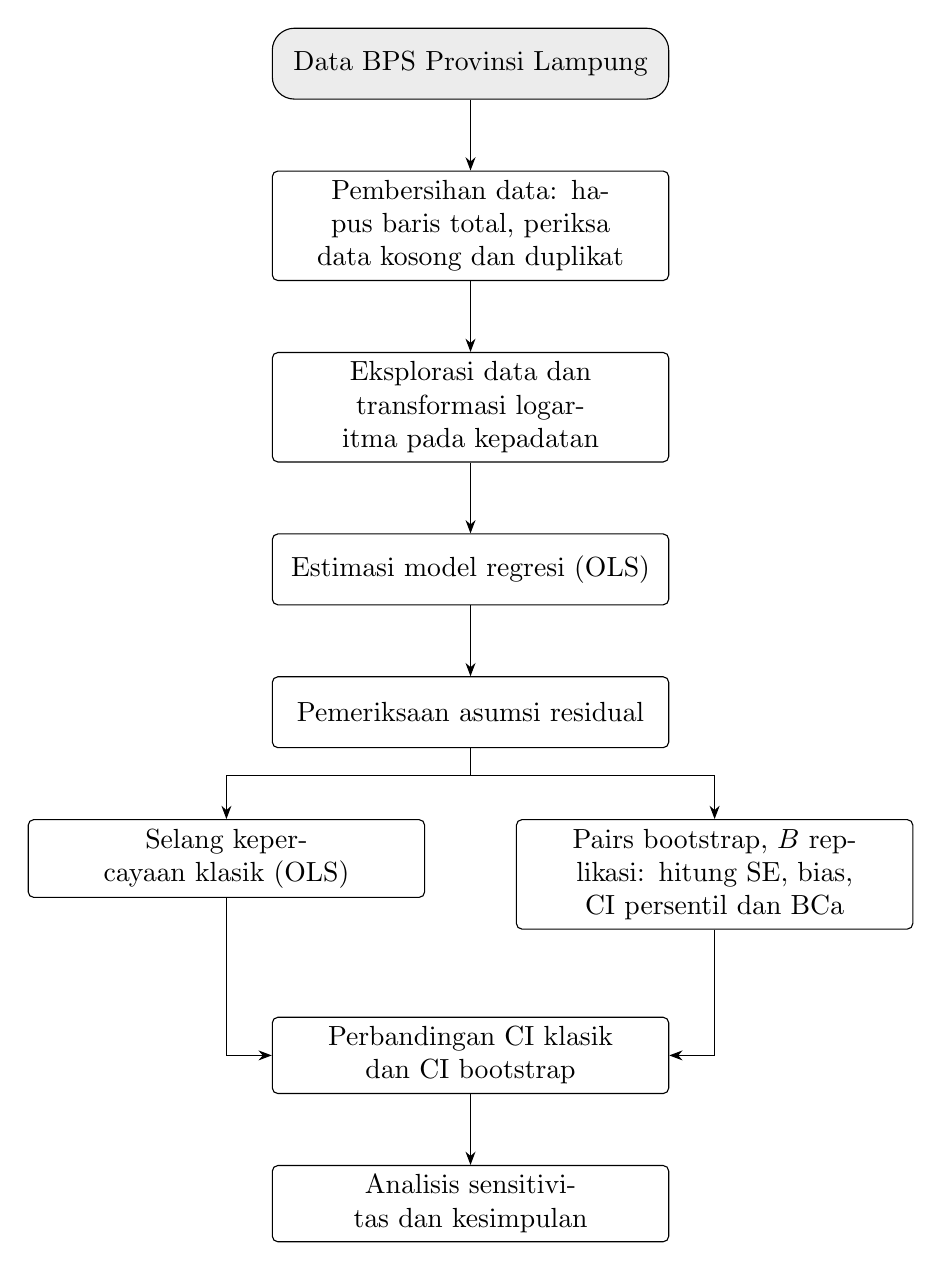
\begin{tikzpicture}[
				node distance=0.9cm, >=Stealth,
				mulai/.style={rectangle, rounded corners=8pt, draw, fill=gray!15,
						align=center, text width=4.8cm, minimum height=0.9cm},
				proses/.style={rectangle, rounded corners=2pt, draw, align=center,
						text width=4.8cm, minimum height=0.9cm}
			]
			\node[mulai]  (a) {Data BPS Provinsi Lampung};
			\node[proses, below=of a] (b) {Pembersihan data: hapus baris total,
				periksa data kosong dan duplikat};
			\node[proses, below=of b] (c) {Eksplorasi data dan transformasi
				logaritma pada kepadatan};
			\node[proses, below=of c] (d) {Estimasi model regresi (OLS)};
			\node[proses, below=of d] (e) {Pemeriksaan asumsi residual};

			\node[proses, below=of e, xshift=-3.1cm] (f1) {Selang kepercayaan klasik (OLS)};
			\node[proses, below=of e, xshift=3.1cm]  (f2) {Pairs bootstrap, $B$ replikasi:
				hitung SE, bias, CI persentil dan BCa};

			\node[proses] (g) at ($(f1)!0.5!(f2)+(0,-2.4)$) {Perbandingan CI klasik
				dan CI bootstrap};
			\node[proses, below=of g] (h) {Analisis sensitivitas dan kesimpulan};

			\draw[->] (a) -- (b);
			\draw[->] (b) -- (c);
			\draw[->] (c) -- (d);
			\draw[->] (d) -- (e);
			\draw[->] (e.south) -- ++(0,-0.35) -| (f1.north);
			\draw[->] (e.south) -- ++(0,-0.35) -| (f2.north);
			\draw[->] (f1.south) |- (g.west);
			\draw[->] (f2.south) |- (g.east);
			\draw[->] (g) -- (h);
		\end{tikzpicture}
		\caption{Alur penelitian}
		\label{fig:alur}
	\end{figure}


	\section{Pembahasan}

	\section{Kesimpulan}
\end{multicols}


\end{document}
